\chapter{遗传密码}
\label{chap:chapter8}
\minitoc

到现在为止,我们已经使用Perl进行了基序的查找、模拟DNA突变、生成随机序列,以及把DNA转录成RNA。这些都是非常重要的主题,它们可以作为你在研究生物学系统过程中使用到的计算技术的好的入门指引。

在本章中,我们将编写Perl程序,来模拟遗传密码是如何指导DNA翻译成蛋白质的。开始我先介绍散列这种数据类型。之后,在对不同的数据结构(散列、数组和数据库)如何对实验信息存取进行简要的讨论后,我们将编写一个程序,来吧DNA翻译成蛋白质。我们也将继续探讨正则表达式,并编写处理FASTA文件的代码。

\section{散列}
在Perl中有三种主要的数据类型。你已经学习了其中的两种:标量变量和数组。现在,我们将开始学习第三种:\textit{散列}(也叫做关联数组)。

散列提供了与键相关联的值的快速查找。举个例子,比如说你有一个叫做\verb|%english_dictionary|的散列。(是的,散列以百分号起始。)如果你想查找单词“recreant”的定义,可以这样:

\begin{lstlisting}
$definition = $english_dictionary{'recreant'};
\end{lstlisting}

标量\verb|'recreant'|是键,返回的标量定义是值。就像你在这个例子中看到的这样,当你访问单个元素时,散列(就像数组那样)把起始的字符换成了美元符号,因为散列查找返回的值是一个标量值。通过它们使用的括号类型,你可以把散列查找和数组元素区分开来:数组使用中括号[ ],而散列使用大括号{ }。

如果你想给键赋值,只需要一个类似的简单语句:

\begin{lstlisting}
$english_dictionary{'recreant'} = "One who calls out in surrender.";
\end{lstlisting}

此外,如果你想用一些键值对初始化一个散列,方法类似于初始化数组,不同的是每一对都成了键-值对:

\begin{lstlisting}
%classification = (
  'dog',      'mammal',
  'robin',    'bird',
  'asp',      'reptile',
);
\end{lstlisting}

它用值\verb|'mammal'|对键\verb|'dog'|进行了初始化,依此类推。还有另一种书写方法,可以使其含义更加清晰一些。下面这些代码所做的事情和前面的代码完全一样,但把键-值的关系表现的更加明确一些:

\begin{lstlisting}
%classification = (
  'dog'   => 'mammal',
  'robin' => 'bird',
  'asp',  => 'reptile',
);
\end{lstlisting}

你可以得到散列的所有键构成的数组:

\begin{lstlisting}
@keys  = keys %my_hash;
\end{lstlisting}

你可以得到散列的所有值构成的数组:

\begin{lstlisting}
@values  = values %my_hash;
\end{lstlisting}

在许多不同的情形下你都会用到散列,尤其是当你的数据以键-值形式存在时,或者你需要快速查找到某个键的值时。举个例子,在本章的后面部分,我们将编写程序,使用散列来提取一个基因的信息。基因的名字就是键,关于基因的信息就是键的值。从数学上来讲,一个Perl散列表示的永远是一个有穷函数。

“散列”这个名字来源于散列函数,如果你留心去寻找,几乎关于算法的任何一本书中都会对它进行定义。让我们跳过它们深层次的工作细节,只讨论它们的表现。

\section{生物学的数据结构和算法}
生物学家研究生物学数据,并且试图阐明在生命系统中基于它的存在结构是如何发挥功能的。生物信息学常被用来尽可能的对这样的存在结构进行建模。(不要太咬文嚼字了,我只是概括而言的!)

生物信息学也会采取略有不同的方案。它会考虑对于这些数据可以做什么,然后尝试去阐明如何对它们进行组织才能实现目标。换句话说,通过以一种方便的数据结构来表征数据,它会尝试去产生一种算法。

既然你已经学习了Perl中的三种数据类型,就是标量、数组和散列,现在是时候来看一下与算法和数据结构相关的主题了。在\autoref{chap:chapter3}中,我们已经讨论了算法。现在讨论的重点就是算法中数据组织形式的重要性,换言之,就是算法中的数据结构。

此处最为关键的一点是,不同的算法通常需要不同的数据结构。

\subsection{基因表达数据库}
让我们考虑一个典型问题。假设你在研究一种生物,它总共大约有30,000个基因。(是的,没错,这就是人类。)假设你正在研究一种类型的细胞,在某个特定的环境条件下它还没有被深入研究过,你想知道,对于每一个基因来说,它是否表达了。\footnote{对于非生物学家:当一个基因转录成RNA后,就可以进一步翻译出蛋白质了,就说这个基因表达了。}你有一个很好的芯片设备,它把那个细胞的表达信息都告诉你了。现在,对于每一个基因,你要去查找一下看看在细胞中它是否表达了。你必须在你的网站上实现这种查找功能,这样在你即将发表的文章中看到你结果的访问者就可以找到基因的表达数据了。

有许多不同的方法可以实现。让我们看一下几个不同的实现方法,作为对算法和数据结构的艺术和科学的简洁的入门介绍。

你的数据是什么?为简单起见,假设你有这个生物所有基因的名字,以及在你的实验中表示表达水平的基因的表达数值。所有未表达的基因的表达数值都是0。

\subsection{使用未排序数组的基因表达数据}
现在,假设你想指导基因是否表达了,而不是具体的表达水平,并且你想使用数组来解决这个编程问题。毕竟,现在你已经对数组非常熟悉了。你该怎么做呢?

你可能只在数组中存储那些表达基因的基因名,而丢弃其他的基因名。假如有8,000个表达基因。之后,要进行任何查询,只需要遍历数组,把查询的基因名和数组中的每一个基因名进行比较,直到你找到它或者没有找到它但已经到达了数组的末尾。

这样是可行的,但也存在问题。最主要的,它非常慢。如果你只是偶尔查询一下,这并不是问题,但如果有许多人访问你的网站对这套新的表达数据进行查询,问题就大了。平均来说,查找一个表达基因需要遍历4,000个基因名字,而查找一个未表达的基因则需要进行8,000此比较。

此外,如果某个人查找的是你的研究中没有的一个基因,因为你丢弃了所有未表达基因的基因名,所以你就没法对其进行回应。查询给出的结果是没有找到这个基因,而不是说要查询的基因并不在你的实验结果中的错误信息。如果要查询的基因虽然并不在你的研究结果中,但却在这类细胞中表达(你刚好错过了它),那这个查询就是一个假阴性了。你可能更希望遇到这种情况时,你的程序可以报告给用户,说那个名字的基因并没有在实验中被研究。

所以你打算把30,000个基因都存储到数组中。(当然,现在进行查找会更慢一些。)但是,如何把表达基因和未表达基因区分开来呢?你可以把每个基因的名字都存储到数组中,并且把表达测量值附加到每个基因名的后面,然后你就可以准确无误的知道某个基因是不是在你的实验中并不存在了。

然而,这个程序仍然有点慢。你仍然不得不去遍历整个数组,直到你找到那个基因或者确定它并没有被研究为止。如果它是数组中的第一个元素,你立马就可找到它,否则你可能不得不等到它遍历到数组的最后一个元素。平均来说,你将不得不遍历一半的数组。另外,你还不得不把需要查找的基因名和数组中的基因名一个一个进行比较。对于每次查询来说,平均都要进行15,000次的比较,这非常慢。(实际上,在现代的计算机上,这其实也并不是慢的可怕。但是我想指出这一点,这样的东西确实意味着一个运行很慢的程序。)

另外一个问题就是,在一个标量中你存储了两个值:基因名和表达测量值。处理这样的数据,你必须还要把基因名和基因的表达测量值分割开来。

虽然有这些缺点,但这种方法确实是可行的。现在,我们来讨论一下另外一种方法。

\subsection{使用排序数组和折半查找的基因表达数据}
你可能尝试把所有的基因名按照字母顺序排序后存储在数组中,然后使用下面这种查找技术。首先,看一下中间的元素。(就像我们已经看到的,使用\verb|scalar @array|表达式你可以得到数组的大小)。按照字母顺序,如果你的基因名排在中间元素的前面,你就可以忽略数组的后半部分了,并找到数组剩余的前半部分的中间元素。如此循环往复,每一步都可以把查找范围缩小到前一步元素数目的一半,直到最终找到对应的匹配,或者发现根本不存在。下面是用伪代码进行实现:

\begin{lstlisting}
Given a sorted array, and an element:

Until you find the element or discover it's not there,

  Pick the midpoint of the array, $array[scalar(@array)/2]

  Compare your element with the element at the midpoint

  If that matches your element, you're done.

  Else, ignore the half of the array that your element is not in
}
\end{lstlisting}

在Perl中要按照字母顺序比较两个字符串,你可以使用\textit{cmp}操作符,如果两个字符串一样它会返回0,如果它们按照字母顺序排列就会返回-1,如果它们按照字母顺序的逆序排列就会返回1。比如,下面这个会返回0:

\begin{lstlisting}
'ZZZ' cmp 'ZZZ';
\end{lstlisting}

这个返回-1:

\begin{lstlisting}
'AAA' cmp 'ZZZ';
\end{lstlisting}

最后,这个返回1:

\begin{lstlisting}
'ZZZ' cmp 'AAA';
\end{lstlisting}

这种算法叫做\textit{折半查找},它会明显提高在数组中进行查找的速度。比如,要查找30,000个基因,最多只需要大约15次的循环即可。(和未排序数组平均进行15,000次的比较相比。)当然,你还必须要对列表进行排序,这也需要一定的时间。如果你需要不停地增加元素,你就不得不把它们插入倒合适的位置,或者把它们添加到末尾然后对整个数组进行重新排序。所有这样的插入或者排序都可能会相当的慢。但是,如果你仅需要进行一次排序,然后进行大量的查找,折半查找还是值得考虑的。

既然我们已经谈到了它,就来看看如何对数据进行排序。这是按照字母顺序对由字符串构成的数组进行排序的方法:

\begin{lstlisting}
@array = sort @array;
\end{lstlisting}

这是以升序对由数字构成的数组进行排序的方法:

\begin{lstlisting}
@array = sort { $a <=> $b  } @array;
\end{lstlisting}

还可以进行多种其他形式的排序,但这些是最常见的。更多的细节,可以参看Perl文档中关于\textit{sort}函数的说明。

\subsection{使用散列的基因表达数据}
你还可以使用散列来查找你数据中的某个基因。要实现这一点,你需要以基因名作为键、以表达测量值作为值载入散列。然后对散列一个简单的调用,使用待查找基因的基因名作为键,就可以返回这个基因的实验结果,这就是你要的答案。与把基因名和表达值存储到一个标量字符串中相比,这个过程要清晰多了。在这里,键是一个标量,而值则是另外一个标量。

此外,取决于散列的构建方式,你可以很快得到你要的答案,因为现在的散列都不需要进行繁琐的查找就可以找到某个键的值。使用散列通常要比折半查找快很多。此外,你还可以知道查找的基因在数据中是否存在,因为你可以明确询问某个散列值是否被定义了,就像这样:

\begin{lstlisting}
if( defined $myhash{'mykey'}  ) { ... }
\end{lstlisting}

另外,如果你开启了警告模式,你会得到一个错误信息,因为你提到的是一个未定义的值。

相比于折半查找,散列的另一个优势在于,你可以向散列中添加或删减元素,而不需要对整个数组进行重排序。

最后,因为散列是作为一个基本的数据类型内置在Perl中的,所以它们非常容易使用,而且你不需要进行太多的编程就可以实现你的目的。通常情况下,节省编程的时间要比节省程序运行的时间更加重要一些。我在\autoref{chap:chapter3}中提到过这一点,但此处还是有必要强调一下。对于一个程序员来说,懒惰的方法通常都是最有效的方法:让机器来干活吧!

但是,不要想当然的认为散列永远都是最好的方法。比如,散列并不以排序的顺序存储其中的元素,所以如果你需要以排序的方式查看数据,就不得不对它进行明确的排序,就像这样:

\begin{lstlisting}
@sorted_keys = sort keys %my_hash;
\end{lstlisting}

这样就可以了,但对于大的数组来说,它可能会有点慢。(当然,你也可以对值进行排序。)

对于这个表达数据的例子,我们总结以下关于数据结构的讨论,下面是对Perl中不同数据结构属性的信息描述,包括对基因名数据集进行的查找、添加和删减、以及保持排序顺序:

\begin{itemize}
  \item 如果你只需要看看某个东西是不是在数据集中,并不需要按照顺序把它们罗列出来,那就使用散列。
  \item 如果你需要一个排序的数据集以及相对快速的查找,而不需要频繁添加或删减元素,使用排序数组结合折半查找就可以了。
  \item
    如果你不需要对元素进行排序,但是需要快速找到最新添加的元素,使用数组并结合Perl函数\textit{push}和\textit{pop}就可以了。
  \item
    如果你不需要对元素进行排序,但是需要添加元素,使用Perl的数组结合函数\textit{push}和\textit{shift}就可以了。当总是需要移除”最老“的元素(待在数组中时间最长的元素)时,这种方案尤其有用。
\end{itemize}

更多信息,可以参看\autoref{chap:chapteraa}和\textit{Mastering Algorithms with Perl}(O'Reilly出版),尤其是后者。

\subsection{关系数据库}
数据库是存储和访问海量数据的程序。它们提供了最常用的数据类型形式在算法中使用。有一些流行的数据库,其中一些非常好的还是免费的(最好的那些都非常昂贵),而Perl提供了对所有最流行数据库的访问方法。比如,Perl/DBI模块,提供了方便的方法,可以在Perl程序中对关系数据库进行访问。

大多数数据库都叫做关系型,这描述了它们存储数据的方式。这种类型数据库的另外一个比较常见的名字是\textit{关系数据库管理系统},简称RDMS。

关系数据库把数组组织成表格进行存储。数据通常通过一种查询语言进行输入和提取,它叫做\textit{结构化查询语言},简称SQL。这是一种非常简单的语言,可以在表格中访问数据,同时跟随表格之间的链接。

关系数据库是存储和提取海量数据最流行的方法,但它们确实需要一定的学习。对关系数据库进行编程已经超出了本书讨论的范畴,但如果你最终需要使用Perl进行大量的编程,你会发现知道使用数据库的基础知识是一个宝贵的技能。参看\autoref{chap:chapter13}中的相关讨论。

尤其是,把你的基因表达数据存储到一个关系数据库中,然后在程序中使用来对网站上的查询做出回应,这完全合情合理。

\subsection{DBM}
Perl有一个简单的、内置的方法来存储散列数据,叫做\textit{数据库管理器}(DBM)。它使用起来非常简单:在启动之后,它把一个散列“绑定”到计算机硬盘上的一个文件,这样你就可以散列保存下来以便日后对其进行重用了。这实际上是一个简单(且非常有用)的数据库。除了初始化以外,你就像使用散列一样使用它。你可以把你的基因和表达数据存储到一个DBM文件中,然后像散列一样使用它。在\autoref{chap:chapter10}中有关于DBM的更多讨论。

\section{遗传密码}
遗传密码就是细胞把包含在DNA中的信息翻译成氨基酸的方式,氨基酸进而形成在细胞中真正发挥功能的蛋白质。

\subsection{背景}
此处是这对非生物学家的简短介绍。

如前所述,DNA编码蛋白质的一级结构(也就是氨基酸序列)。DNA有四种核苷酸,而蛋白质有20种氨基酸。编码的过程就是从DNA中找到三个核苷酸,把它们作为一组“翻译”成一个氨基酸或者终止信号。这样每一组的三个核苷酸叫做\textit{密码子}。稍后我们将会看到编码和翻译过程的细节。

事实上,\textit{转录}首先利用DNA制造RNA,然后\textit{翻译}再利用RNA制造蛋白质。这就是分子生物学的\textit{中心法则}。但是,在本课程中,我将把从DNA到蛋白质的整个过程不准确地简称为“翻译”。

之所以要进行这样的区分,是因为通过使用字符串来表征DNA、RNA和蛋白质,在计算机中可以非常简单的对整个过程进行模拟。事实上,就像在\autoref{chap:chapter4}中演示的那样,把DNA转录成RNA确实非常简单。在你的计算机模拟中,可以简单的跳过这一步,因为它只不过是把一个字母换成了另一个字母而已。(当然,细胞中的真实过程要复杂得多。)

注意,使用四种碱基,DNA的每三个碱基构成一组,这样可以表征4 x 4 x 4 = 64可能的氨基酸。因为只有20种氨基酸外加一个终止信号,遗传密码进化出了冗余性,所以某些氨基酸由不止一个密码子所表征。每一种可能的DNA三碱基——每一个密码子——都表征某个氨基酸(除了三个密码子表征终止信号外)。

\autoref{fig:figure8.1}中的表格演示了不同的碱基是如何组合形成一个氨基酸的。对于遗传密码,有一些有趣的现象需要注意一下。对于我们的目的来说,最重要的就是冗余性——不止一个密码子翻译成同一个氨基酸。很快腻就会看到,我们将使用字符类和正则表达式对其进行编程。\footnote{此外,还要注意\autoref{fig:figure8.1}中的遗传密码是基于RNA的,尿嘧啶替代胸腺嘧啶出现在了其中。在我们的程序中,我们将直接把DNA翻译成氨基酸,所以我们的代码中将使用胸腺嘧啶而不是尿嘧啶。}

\begin{figure}
  \centering
  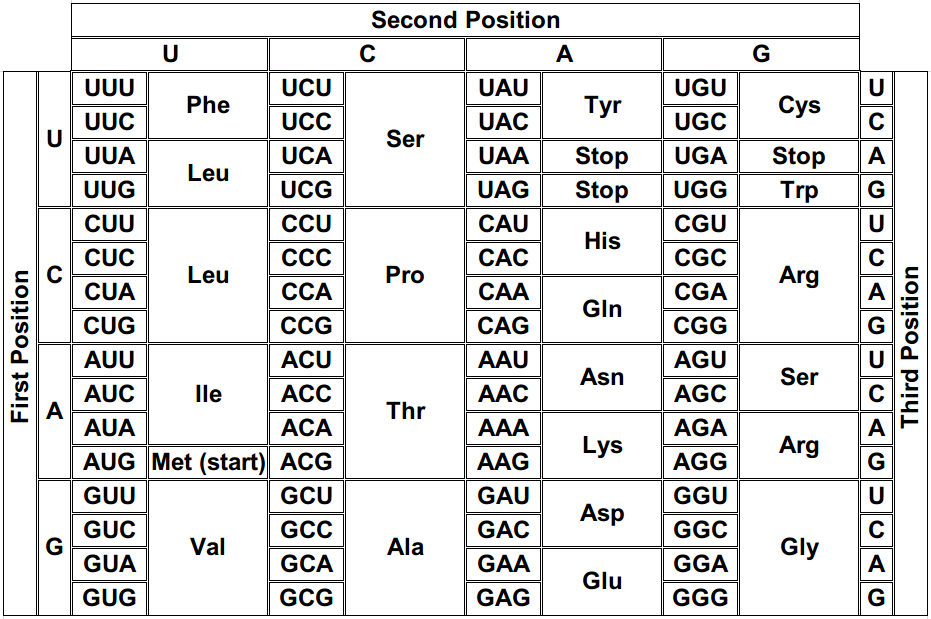
\includegraphics[width=13cm]{figure8.1.png}
  \caption{遗传密码}
  \label{fig:figure8.1}
\end{figure}

细胞中的翻译机器实际上会从RNA的某处起始,并“读取”一个接一个的密码子,把编码的氨基酸附加到不断增长的蛋白质序列的尾部。\autoref{exam:example8.1}模拟了这个过程,一次读取DNA字符串的三个碱基,然后把编码的氨基酸符号串联到不断增长的蛋白质字符串的尾部。在细胞中,当遇到三个终止密码子中的任意一个时,这个过程就会停止。

\subsection{把密码子翻译成氨基酸}
The first task is to enable the following programs to do the translation from the three-nucleotide codons to the amino acids. This is the most important step in implementing the genetic code, which is the encoding of amino acids by three-nucleotide codons.

Here's a subroutine that returns an amino acid (represented by a one-letter abbreviation) given a three-letter DNA codon: 

\begin{lstlisting}
# codon2aa
#
# A subroutine to translate a DNA 3-character codon to an amino acid

sub codon2aa {
  my($codon) = @_;
    
     if ( $codon =~ /TCA/i )    { return 'S' }    # Serine
  elsif ( $codon =~ /TCC/i )    { return 'S' }    # Serine
  elsif ( $codon =~ /TCG/i )    { return 'S' }    # Serine
  elsif ( $codon =~ /TCT/i )    { return 'S' }    # Serine
  elsif ( $codon =~ /TTC/i )    { return 'F' }    # Phenylalanine
  elsif ( $codon =~ /TTT/i )    { return 'F' }    # Phenylalanine
  elsif ( $codon =~ /TTA/i )    { return 'L' }    # Leucine
  elsif ( $codon =~ /TTG/i )    { return 'L' }    # Leucine
  elsif ( $codon =~ /TAC/i )    { return 'Y' }    # Tyrosine
  elsif ( $codon =~ /TAT/i )    { return 'Y' }    # Tyrosine
  elsif ( $codon =~ /TAA/i )    { return '_' }    # Stop
  elsif ( $codon =~ /TAG/i )    { return '_' }    # Stop
  elsif ( $codon =~ /TGC/i )    { return 'C' }    # Cysteine
  elsif ( $codon =~ /TGT/i )    { return 'C' }    # Cysteine
  elsif ( $codon =~ /TGA/i )    { return '_' }    # Stop
  elsif ( $codon =~ /TGG/i )    { return 'W' }    # Tryptophan
  elsif ( $codon =~ /CTA/i )    { return 'L' }    # Leucine
  elsif ( $codon =~ /CTC/i )    { return 'L' }    # Leucine
  elsif ( $codon =~ /CTG/i )    { return 'L' }    # Leucine
  elsif ( $codon =~ /CTT/i )    { return 'L' }    # Leucine
  elsif ( $codon =~ /CCA/i )    { return 'P' }    # Proline
  elsif ( $codon =~ /CCC/i )    { return 'P' }    # Proline
  elsif ( $codon =~ /CCG/i )    { return 'P' }    # Proline
  elsif ( $codon =~ /CCT/i )    { return 'P' }    # Proline
  elsif ( $codon =~ /CAC/i )    { return 'H' }    # Histidine
  elsif ( $codon =~ /CAT/i )    { return 'H' }    # Histidine
  elsif ( $codon =~ /CAA/i )    { return 'Q' }    # Glutamine
  elsif ( $codon =~ /CAG/i )    { return 'Q' }    # Glutamine
  elsif ( $codon =~ /CGA/i )    { return 'R' }    # Arginine
  elsif ( $codon =~ /CGC/i )    { return 'R' }    # Arginine
  elsif ( $codon =~ /CGG/i )    { return 'R' }    # Arginine
  elsif ( $codon =~ /CGT/i )    { return 'R' }    # Arginine
  elsif ( $codon =~ /ATA/i )    { return 'I' }    # Isoleucine
  elsif ( $codon =~ /ATC/i )    { return 'I' }    # Isoleucine
  elsif ( $codon =~ /ATT/i )    { return 'I' }    # Isoleucine
  elsif ( $codon =~ /ATG/i )    { return 'M' }    # Methionine
  elsif ( $codon =~ /ACA/i )    { return 'T' }    # Threonine
  elsif ( $codon =~ /ACC/i )    { return 'T' }    # Threonine
  elsif ( $codon =~ /ACG/i )    { return 'T' }    # Threonine
  elsif ( $codon =~ /ACT/i )    { return 'T' }    # Threonine
  elsif ( $codon =~ /AAC/i )    { return 'N' }    # Asparagine
  elsif ( $codon =~ /AAT/i )    { return 'N' }    # Asparagine
  elsif ( $codon =~ /AAA/i )    { return 'K' }    # Lysine
  elsif ( $codon =~ /AAG/i )    { return 'K' }    # Lysine
  elsif ( $codon =~ /AGC/i )    { return 'S' }    # Serine
  elsif ( $codon =~ /AGT/i )    { return 'S' }    # Serine
  elsif ( $codon =~ /AGA/i )    { return 'R' }    # Arginine
  elsif ( $codon =~ /AGG/i )    { return 'R' }    # Arginine
  elsif ( $codon =~ /GTA/i )    { return 'V' }    # Valine
  elsif ( $codon =~ /GTC/i )    { return 'V' }    # Valine
  elsif ( $codon =~ /GTG/i )    { return 'V' }    # Valine
  elsif ( $codon =~ /GTT/i )    { return 'V' }    # Valine
  elsif ( $codon =~ /GCA/i )    { return 'A' }    # Alanine
  elsif ( $codon =~ /GCC/i )    { return 'A' }    # Alanine
  elsif ( $codon =~ /GCG/i )    { return 'A' }    # Alanine
  elsif ( $codon =~ /GCT/i )    { return 'A' }    # Alanine
  elsif ( $codon =~ /GAC/i )    { return 'D' }    # Aspartic Acid
  elsif ( $codon =~ /GAT/i )    { return 'D' }    # Aspartic Acid
  elsif ( $codon =~ /GAA/i )    { return 'E' }    # Glutamic Acid
  elsif ( $codon =~ /GAG/i )    { return 'E' }    # Glutamic Acid
  elsif ( $codon =~ /GGA/i )    { return 'G' }    # Glycine
  elsif ( $codon =~ /GGC/i )    { return 'G' }    # Glycine
  elsif ( $codon =~ /GGG/i )    { return 'G' }    # Glycine
  elsif ( $codon =~ /GGT/i )    { return 'G' }    # Glycine
  else {
    print STDERR "Bad codon \"$codon\"!!\n";
    exit;
  }
}
\end{lstlisting}

This code is clear and simple, and the layout makes it obvious what's happening. However, it can take a while to run. For instance, given the codon GGT for glycine, it has to check each test until it finally succeeds on the last one, and that's a lot of string comparisons. Still, the code achieves its purpose.

There's something new happening in the code's error message. Recall filehandles from \autoref{chap:chapter4} and how they access data in files. From \autoref{chap:chapter5}, remember the special filehandle STDIN that reads user input from the keyboard. STDOUT and STDERR are also special filehandles that are always available to Perl programs. STDOUT directs output to the screen (usually) or another standard place. When a filehandle is missing from a \verb|print| statement, STDOUT is assumed. The \textit{print} statement accepts a filehandle as an optional argument, but so far, we've been printing to the default STDOUT. Here, error messages are directed to STDERR, which usually prints to the screen, but on many computer systems they can be directed to a special error file or other location. Alternatively, you sometimes want to direct STDOUT to a file or elsewhere but want STDERR error messages to appear on your screen. I mention these options because you are likely to come across them in Perl code; we don't use them much in this book (see \autoref{chap:chapterab} for more information).  

\subsection{The Redundancy of the Genetic Code}
I've remarked on the redundancy of the genetic code, and the last subroutine clearly displays this redundancy. It might be interesting to express that in your subroutine. Notice that groups of redundant codons almost always have the same first and second bases and vary in the third. You've used character classes in regular expressions to match any of a set of characters. Now, let's try to redo the subroutine to make one test for each redundant group of codons: 

\begin{lstlisting}
# codon2aa
#
# A subroutine to translate a DNA 3-character codon to an amino acid
#   Version 2

sub codon2aa {
  my($codon) = @_;
 
     if ( $codon =~ /GC./i)        { return 'A' }    # Alanine
  elsif ( $codon =~ /TG[TC]/i)     { return 'C' }    # Cysteine
  elsif ( $codon =~ /GA[TC]/i)     { return 'D' }    # Aspartic Acid
  elsif ( $codon =~ /GA[AG]/i)     { return 'E' }    # Glutamic Acid
  elsif ( $codon =~ /TT[TC]/i)     { return 'F' }    # Phenylalanine
  elsif ( $codon =~ /GG./i)        { return 'G' }    # Glycine
  elsif ( $codon =~ /CA[TC]/i)     { return 'H' }    # Histidine
  elsif ( $codon =~ /AT[TCA]/i)    { return 'I' }    # Isoleucine
  elsif ( $codon =~ /AA[AG]/i)     { return 'K' }    # Lysine
  elsif ( $codon =~ /TT[AG]|CT./i) { return 'L' }    # Leucine
  elsif ( $codon =~ /ATG/i)        { return 'M' }    # Methionine
  elsif ( $codon =~ /AA[TC]/i)     { return 'N' }    # Asparagine
  elsif ( $codon =~ /CC./i)        { return 'P' }    # Proline
  elsif ( $codon =~ /CA[AG]/i)     { return 'Q' }    # Glutamine
  elsif ( $codon =~ /CG.|AG[AG]/i) { return 'R' }    # Arginine
  elsif ( $codon =~ /TC.|AG[TC]/i) { return 'S' }    # Serine
  elsif ( $codon =~ /AC./i)        { return 'T' }    # Threonine
  elsif ( $codon =~ /GT./i)        { return 'V' }    # Valine
  elsif ( $codon =~ /TGG/i)        { return 'W' }    # Tryptophan
  elsif ( $codon =~ /TA[TC]/i)     { return 'Y' }    # Tyrosine
  elsif ( $codon =~ /TA[AG]|TGA/i) { return '_' }    # Stop
  else {
    print STDERR "Bad codon \"$codon\"!!\n";
    exit;
  }
}
\end{lstlisting}

Using character classes and regular expressions, this code clearly shows the redundancy of the genetic code. Also notice that the one-character codes for the amino acids are now in alphabetical order. 

A character class such as \verb|[TC]| matches a single character, either T or C. The \verb|.| is the regular expression that matches any character except a newline. The \verb|/GT./i| expression for valine matches GTA, GTC, GTG, and GTT, all of which are codons for valine. (Of course, the period matches any other character, but the \verb|$codon| is assumed to have only A,C,G, or T characters.) The i after the regular expression means match uppercase or lowercase, for instance \verb|/T/i| matches T or t.

The new feature in these regular expressions is the use of the vertical bar or pipe (|) to separate two choices. Thus for serine, \verb=/TC.|AG[TC]/= matches \verb|/TC./| or \verb|/AG[TC]/|. In this program, you need only two choices per regular expression, but you can use as many vertical bars as you like.

You can also group parts of a regular expression in parentheses, and use vertical bars in them. For example, \verb=/give me a (break|meal)/= matches "give me a break" or "give me a meal." 

\subsection{Using Hashes for the Genetic Code}
If you think about using a hash for this translation, you'll see it's a natural way to proceed. For each codon key the amino acid value is returned. Here's the code: 

\begin{lstlisting}
#
# codon2aa
#
# A subroutine to translate a DNA 3-character codon to an amino acid
#   Version 3, using hash lookup

sub codon2aa {
  my($codon) = @_;

  $codon = uc $codon;
 
  my(%genetic_code) = (
  
  'TCA' => 'S',    # Serine
  'TCC' => 'S',    # Serine
  'TCG' => 'S',    # Serine
  'TCT' => 'S',    # Serine
  'TTC' => 'F',    # Phenylalanine
  'TTT' => 'F',    # Phenylalanine
  'TTA' => 'L',    # Leucine
  'TTG' => 'L',    # Leucine
  'TAC' => 'Y',    # Tyrosine
  'TAT' => 'Y',    # Tyrosine
  'TAA' => '_',    # Stop
  'TAG' => '_',    # Stop
  'TGC' => 'C',    # Cysteine
  'TGT' => 'C',    # Cysteine
  'TGA' => '_',    # Stop
  'TGG' => 'W',    # Tryptophan
  'CTA' => 'L',    # Leucine
  'CTC' => 'L',    # Leucine
  'CTG' => 'L',    # Leucine
  'CTT' => 'L',    # Leucine
  'CCA' => 'P',    # Proline
  'CCC' => 'P',    # Proline
  'CCG' => 'P',    # Proline
  'CCT' => 'P',    # Proline
  'CAC' => 'H',    # Histidine
  'CAT' => 'H',    # Histidine
  'CAA' => 'Q',    # Glutamine
  'CAG' => 'Q',    # Glutamine
  'CGA' => 'R',    # Arginine
  'CGC' => 'R',    # Arginine
  'CGG' => 'R',    # Arginine
  'CGT' => 'R',    # Arginine
  'ATA' => 'I',    # Isoleucine
  'ATC' => 'I',    # Isoleucine
  'ATT' => 'I',    # Isoleucine
  'ATG' => 'M',    # Methionine
  'ACA' => 'T',    # Threonine
  'ACC' => 'T',    # Threonine
  'ACG' => 'T',    # Threonine
  'ACT' => 'T',    # Threonine
  'AAC' => 'N',    # Asparagine
  'AAT' => 'N',    # Asparagine
  'AAA' => 'K',    # Lysine
  'AAG' => 'K',    # Lysine
  'AGC' => 'S',    # Serine
  'AGT' => 'S',    # Serine
  'AGA' => 'R',    # Arginine
  'AGG' => 'R',    # Arginine
  'GTA' => 'V',    # Valine
  'GTC' => 'V',    # Valine
  'GTG' => 'V',    # Valine
  'GTT' => 'V',    # Valine
  'GCA' => 'A',    # Alanine
  'GCC' => 'A',    # Alanine
  'GCG' => 'A',    # Alanine
  'GCT' => 'A',    # Alanine
  'GAC' => 'D',    # Aspartic Acid
  'GAT' => 'D',    # Aspartic Acid
  'GAA' => 'E',    # Glutamic Acid
  'GAG' => 'E',    # Glutamic Acid
  'GGA' => 'G',    # Glycine
  'GGC' => 'G',    # Glycine
  'GGG' => 'G',    # Glycine
  'GGT' => 'G',    # Glycine
  );

  if(exists $genetic_code{$codon}) {
    return $genetic_code{$codon};
  }else{

    print STDERR "Bad codon \"$codon\"!!\n";
    exit;
  }
}
\end{lstlisting}

This subroutine is simple: it initializes a hash and then performs a single lookup of its single argument in the hash. The hash has 64 keys, one for each codon.

Notice there's a function exists that returns \verb|true| if the key \verb|$codon| exists in the hash. It's equivalent to the \textit{else} statement in the two previous versions of the codon2aa subroutine.\footnote{A key might exist in a hash, but its value can be undefined.  The defined function checks for defined values. Also, of course, the value might be 0 or the empty string, in which case, it fails a test such as \verb|if ($hash{$key}|) because, even though the key exists and the value is defined, the value evaluates to \verb|false| in a conditional test.}

Also notice that to make this subroutine work on lowercase DNA as well as uppercase, you translate the incoming argument into uppercase to match the data in the \verb|%genetic_code| hash. You can't give a regular expression to a hash as a key; it must be a simple scalar value, such as a string or a number, so the case translation must be done first.  (Alternatively, you can make the hash twice as big.) Similarly, character classes don't work in the keys for hashes, so you have to specify each one of the 64 codons individually.

You may wonder why bother wrapping this last bit of code in a subroutine at all. Why not just declare and initialize the hash and do the lookups directly in the hash instead of going through the subroutine? Well, the subroutine does do a little bit of error checking for nonexistent keys, so having a subroutine saves doing that error checking yourself each time you use the hash.

Additionally, wrapping the code in a subroutine gives a little insurance for the future. If all the code you write does codon translation by means of our subroutine, it would be simplicity itself to switch over to a new way of doing the translation. Perhaps a new kind of datatype will be added to Perl in the future, or perhaps you want to do lookups from a database or a DBM file. Then all you have to do is change the internals of this one subroutine. As long as the interface to the subroutine remains the same—that is to say, as long as it still takes one codon as an argument and returns a one-character amino acid—you don't need to worry about how it accomplishes the translation from the standpoint of the rest of the programs. Our subroutine has become a \textit{black box}. This is one significant benefit of modularization and organization of programs with subroutines. 

There's another good, and biological, reason why you should use a subroutine for the genetic code. There is actually more than one genetic code, because there are differences as to how DNA encodes amino acids among mammals, plants, insects, and yeast—especially in the mitochondria. So if you have modularized the genetic code, you can easily modify your program to work with a range of organisms.

One of the benefits of hashes is that they are fast. Unfortunately, our subroutine declares the whole hash each time the subroutine is called, even for one lookup. This isn't so efficient; in fact, it's kind of slow. There are other, much faster ways that involve declaring the genetic code hash only once as a global variable, but they would take us a little far afield at this point. Our current version has the advantage of being easy to read. So, let's be officially happy with the hash version of codon2aa and put it into our module in the file \textit{BeginPerlBioinfo.pm} (see \autoref{chap:chapter6}).

Now that we've got a satisfactory way to translate codons to amino acids, we'll start to use it in the next section and in the examples. 

\section{Translating DNA into Proteins}
\autoref{exam:example8.1} shows how the new \textit{codon2aa} subroutine translates a whole DNA sequence into protein. 

\textbf{Example 8-1. Translate DNA into protein }
\lstinputlisting[label=exam:example8.1]{./scripts/example8-1.pl}

To make this work, you'll need the \textit{BeginPerlBioinfo.pm} module for your subroutines in a separate file the program can find, as discussed in \autoref{chap:chapter6}. You also have to add the \textit{codon2aa} subroutine to it.  Alternatively, you can add the code for the subroutine \textit{condon2aa} directly to the program in \autoref{exam:example8.1} and remove the reference to the \textit{BeginPerlBioinfo.pm} module.

Here's the output from \autoref{exam:example8.1}:

\begin{lstlisting}
I translated the DNA

CGACGTCTTCGTACGGGACTAGCTCGTGTCGGTCGC

  into the protein

RRLRTGLARVGR
\end{lstlisting}

You've seen all the elements in i\autoref{exam:example8.1} before, except for the way it loops through the DNA with this statement:

\begin{lstlisting}
for(my $i=0; $i < (length($dna) - 2) ; $i += 3) {
\end{lstlisting}

Recall that a \verb|for| loop has three parts, delimited by the two semicolons.  The first part initializes a counter: \verb|my $i=0| statically scopes the \verb|$i| variable so it's visible only inside this block, and any other \verb|$i| elsewhere in the code (well, in this case, there aren't any, but it can happen) is now invisible inside the block. The third part of the \verb|for| loop increments the counter after all the statements in the block are executed and before returning to the beginning of the loop:

\begin{lstlisting}
$i += 3
\end{lstlisting}

Since you're trying to march through the DNA three bases at a shot, you increment by three.

The second, middle part of the \verb|for| loop tests whether the loop should continue:

\begin{lstlisting}
$i < (length($dna) - 2)
\end{lstlisting}

The point is that if there are none, one, or two bases left, you should quit, because there's not enough to make a codon. Now, the positions in a string of DNA of a certain length are numbered from \verb|0| to \verb|length-1|. So if the position counter \verb|$i| has reached \verb|length-2|, there's only two more bases (at positions \verb|length-2| and \verb|length-1|), and you should quit. Only if the position counter \verb|$i| is less than \verb|length-2| will you still have at least three bases left, enough for a codon. So the test succeeds only if:

\begin{lstlisting}
$i < (length($dna) -2)
\end{lstlisting}

(Notice also how the whole expression to the right of the less-than sign is enclosed in parentheses; we'll discuss this in \autoref{chap:chapter9} in \autoref{sect:section9.3.1})

The line of code:

\begin{lstlisting}
$codon = substr ($dna, $i 3);
\end{lstlisting}

actually extracts the 3-base codon from the DNA. The call to the \verb|substr| function specifies a substring of \verb|$dna| at position \verb|$i| of length \verb|3|, and saves it in the variable \verb|$codon|. 

If you know you'll need to do this DNA-to-protein translation a lot, you can turn \autoref{exam:example8.1} into a subroutine. Whenever you write a subroutine, you have to think about which arguments you may want to give the subroutine. So you realize, there may come a time when you'll have some large DNA sequence but only want to translate a given part of it. Should you add two arguments to the subroutine as beginning and end points? You could, but decide not to. It's a judgment call—part of the art of decomposing a collection of code into useful fragments. But it might be better to have a subroutine that just translates; then you can make it part of a larger subroutine that picks endpoints in the sequence, if needed. The thinking is that you'll usually just translate the whole thing and always typing in \verb|0| for the start and \verb|length($dna)-1| at the end, would be an annoyance. Of course, this depends on what you're doing, so this particular choice just illustrates your thinking when you write the code.

You should also remove the informative \verb|print| statement at the end, because it's more suited to a main program than a subroutine.

Anyway, you've now thought through the design and just want a subroutine that takes one argument containing DNA and returns a peptide translation: 

\begin{lstlisting}
# dna2peptide 
#
# A subroutine to translate DNA sequence into a peptide

sub dna2peptide {
  
  my($dna) = @_;

  use strict;
  use warnings;
  use BeginPerlBioinfo;     # see Chapter 6 about this module

  # Initialize variables
  my $protein = '';

  # Translate each three-base codon to an amino acid, and append to a protein 
  for(my $i=0; $i < (length($dna) - 2) ; $i += 3) {
    $protein .= codon2aa( substr($dna,$i,3));
  }

  return $protein;
  }
\end{lstlisting}

Now add subroutine \textit{dna2peptide} to the \textit{BeginPerlBioinfo.pm} module.

Notice that you've eliminated one of the variables in making the subroutine out of \autoref{exam:example8.1}: the variable \verb|$codon|. Why?

Well, one reason is because you can. In \autoref{exam:example8.1}, you were using substr to extract the codon from \verb|$dna|, saving it in variable \verb|$codon| and then passing it into the subroutine codon2aa. This new way eliminates the middleman. Put the call to \textit{substr} that extracts the codon as the argument to the subroutine codon2aa so that the value is passed in just as before, but without having to copy it to the variable \verb|$codon| first. 

This has somewhat improved efficiency and speed. Since copying strings is one of the slower things computer programs do, eliminating a bunch of string copies is an easy and effective way to speed up a program.

But has it made the program less readable? You be the judge. I think it has, a little, but the comment right before the loop seems to make everything clear enough, for me, anyway. It's important to have readable code, so if you really need to boost the speed of a subroutine, but find it makes the code harder to read, be sure to include enough comments for the reader to be able to understand what's going on.

For the first time \textit{use} function calls are being included in a subroutine instead of the main program:

\begin{lstlisting}
use strict;
use warnings;
use BeginPerlBioinfo;
\end{lstlisting}

This may be redundant with the calls in the main program, but it doesn't do any harm (Perl checks and loads a module only once). If this subroutine should be called from a module that doesn't already load the modules, it's done some good after all.

Now let's improve how we deal with DNA in files. 

\section{Reading DNA from Files in FASTA Format}
Over the fairly short history of bioinformatics, several different biologists and programmers invented several ways to format sequence data in computer files, and so bioinformaticians must deal with these different formats. We need to extract the sequence data and the annotations from these files, which requires writing code to deal with each different format.

There are many such formats, perhaps as many as 20 in regular use for DNA alone. The very multiplicity of these formats can be an annoyance when you're analyzing a sequence in the lab: it becomes necessary to translate from one format to another for the various programs you use to examine the sequence. Here are some of the most popular: 

\textcolor{red}{\textit{FASTA}}
\begin{adjustwidth}{1cm}{}
The FASTA and Basic Local Alignment Search Technique (BLAST) programs are popular; they both use the FASTA format. Because of its simplicity, the FASTA format is perhaps the most widely used of all formats, aside from GenBank. 
\end{adjustwidth}

\textcolor{red}{\textit{Genetic Sequence Data Bank (GenBank)}}
\begin{adjustwidth}{1cm}{}
GenBank is a collection of all publicly released genetic data. It includes lots of information in addition to the DNA sequence. It's very important, and we'll be looking closely at GenBank files in \autoref{chap:chapter10}. 
\end{adjustwidth}

\textcolor{red}{\textit{European Molecular Biology Laboratory (EMBL)}}
\begin{adjustwidth}{1cm}{}
The EMBL database has substantially the same data as the GenBank and the DDBJ (DNA Data Bank of Japan), but the format is somewhat different. 
\end{adjustwidth}

\textcolor{red}{\textit{Simple data, or Applied Biosystems (ABI) sequencer output}}
\begin{adjustwidth}{1cm}{}
This is DNA sequence data that has no formatting whatsoever, just the characters that represent the bases; it is output into files by the sequencing machines from ABI and from other machines and programs. 
\end{adjustwidth}

\textcolor{red}{\textit{Protein Identification Resource (PIR)}}
\begin{adjustwidth}{1cm}{}
PIR is a well-curated collection of protein sequence data.
\end{adjustwidth}

\textcolor{red}{\textit{Genetics Computer Group (GCG)}}
\begin{adjustwidth}{1cm}{}
The GCG program (a.k.a. the GCG Wisconsin package) from Accelrys is used at many large research institutions. Data must be in GCG format to be usable by their programs. 
\end{adjustwidth}

Of these six sequence formats, GenBank and FASTA are by far the most common. The next few sections take you through the process of reading and manipulating data in FASTA. 

\subsection{FASTA Format}
Let's write a subroutine that can handle FASTA-style data. This is useful in its own right and as a warm-up for the upcoming chapters on GenBank, PDB, and BLAST.

FASTA format is basically just lines of sequence data with newlines at the end so it can be printed on a page or displayed on a computer screen. The length of the lines isn't specified, but for compatibility, it's best to limit them to 80 characters in length. There is also \textit{header information}, a line or lines at the beginning of the file that start with the greater-than > character, that can contain any text whatsoever (or no text). Typically, a header line contains the name of the DNA or the gene it comes from, often separated by a vertical bar from additional information about the sequence, the experiment that produced it, or other, nonsequence information of that nature.

Much FASTA-aware software insists that there must be only one header line; others permit several lines. Our subroutine will accept either one or several header lines plus comments beginning with \#.

The following is a FASTA file. We'll call it sample.dna and use it in several programs. You should copy it, download it from this book's web site, or make up your own file with your own data. 

\begin{lstlisting}
> sample dna | (This is a typical fasta header.)
agatggcggcgctgaggggtcttgggggctctaggccggccacctactgg
tttgcagcggagacgacgcatggggcctgcgcaataggagtacgctgcct
gggaggcgtgactagaagcggaagtagttgtgggcgcctttgcaaccgcc
tgggacgccgccgagtggtctgtgcaggttcgcgggtcgctggcgggggt
cgtgagggagtgcgccgggagcggagatatggagggagatggttcagacc
cagagcctccagatgccggggaggacagcaagtccgagaatggggagaat
gcgcccatctactgcatctgccgcaaaccggacatcaactgcttcatgat
cgggtgtgacaactgcaatgagtggttccatggggactgcatccggatca
ctgagaagatggccaaggccatccgggagtggtactgtcgggagtgcaga
gagaaagaccccaagctagagattcgctatcggcacaagaagtcacggga
gcgggatggcaatgagcgggacagcagtgagccccgggatgagggtggag
ggcgcaagaggcctgtccctgatccagacctgcagcgccgggcagggtca
gggacaggggttggggccatgcttgctcggggctctgcttcgccccacaa
atcctctccgcagcccttggtggccacacccagccagcatcaccagcagc
agcagcagcagatcaaacggtcagcccgcatgtgtggtgagtgtgaggca
tgtcggcgcactgaggactgtggtcactgtgatttctgtcgggacatgaa
gaagttcgggggccccaacaagatccggcagaagtgccggctgcgccagt
gccagctgcgggcccgggaatcgtacaagtacttcccttcctcgctctca
ccagtgacgccctcagagtccctgccaaggccccgccggccactgcccac
ccaacagcagccacagccatcacagaagttagggcgcatccgtgaagatg
agggggcagtggcgtcatcaacagtcaaggagcctcctgaggctacagcc
acacctgagccactctcagatgaggaccta
\end{lstlisting}

\subsection{A Design to Read FASTA Files}
In \autoref{chap:chapter4}, you learned how to read in sequence data; here, you just have to extend that method to deal with the header lines.  You'll also learn how to discard empty lines and lines that begin with the pound sign \#, i.e., comments in Perl and other languages and file formats. (These don't appear in the FASTA file \textit{sample.dna} just shown.)

There are two choices when reading in the data. You can read from the open file one line at a time, making decisions as you go. Or, you can slurp the whole file into an array and then operate on the array. For very big files, it's sometimes best to read them one line at a time, especially if you're looking for some small bit of information. (This is because reading a large file into an array uses a large amount of memory. If your system isn't robust enough, it may crash.)

For smaller, normal-sized files, the advantage to reading all the data into an array is that you can then easily look through at the data and do operations on it. That's what we'll do with our subroutine, but remember, this approach can cause memory space problems with larger files, and there are other ways of proceeding.

Let's write a subroutine that, given as an argument a filename containing FASTA-formatted data, returns the sequence data.

Before doing so you should think about whether you should have just one subroutine, or perhaps one subroutine that opens and reads a file, called by another subroutine that extracts the sequence data. Let's use two subroutines, keeping in mind that you can reuse the subroutine that deals with arbitrary files every time you need to write such a program for other formats.

Let's start with some pseudocode:

\begin{lstlisting}
subroutine get data from a file

  argument = filename

  open file
    if can't open, print error message and exit

  read in data and 

  return @data
}

Subroutine extract sequence data from fasta file

  argument = array of file data in fasta format

    Discard all header lines
    (and blank and comment lines for good measure)
    If first character of first line is >, discard it

  Read in the rest of the file, join in a scalar,
    edit out nonsequence data

  return sequence
}
\end{lstlisting}

In the first subroutine that gets data from a file, there's a question as to what's the best thing to do when the file can't be read. Here, we're taking the drastic approach: yelling "Fire!" and exiting. But you wouldn't necessarily want your program to just stop whenever it can't open a file. Maybe you're asking for filenames from the user at the keyboard or on a web page, and you'd like to give them three chances to type in the filename correctly. Or maybe, if the file can't be opened, you want a default file instead.

Maybe you can return a \verb|false| value, such as an empty array, if you can't open the file. Then a program that calls this subroutine can exit, try again, or whatever it wants. But what if you successfully open the file, but it was absolutely empty? Then you'd have succeeded and returned an empty array, and the program calling this subroutine would think incorrectly, that the file couldn't be opened. So, that wouldn't work.

There are other options, such as returning the special "undefined" value. Let's keep what we've got, but it's important to remember that handling errors can be an important, and sometimes tricky, part of writing \textit{robust code}, code that responds well in unusual circumstances.

The second subroutine takes the array of FASTA-formatted sequence and returns just the unformatted sequence in a string. 

\subsection{A Subroutine to Read FASTA Files}
Now that you've thought about the problem, written some pseudocode, considered alternate ways of designing the subroutines and the costs and benefits of the choices, you're ready to code:

\begin{lstlisting}
# get_file_data
#
# A subroutine to get data from a file given its filename

sub get_file_data {

  my($filename) = @_;

  use strict;
  use warnings;

  # Initialize variables
  my @filedata = (  );

  unless( open(GET_FILE_DATA, $filename) ) {
    print STDERR "Cannot open file \"$filename\"\n\n";
    exit;
  }

  @filedata = <GET_FILE_DATA>;

  close GET_FILE_DATA;

  return @filedata;
}

# extract_sequence_from_fasta_data
#
# A subroutine to extract FASTA sequence data from an array

sub extract_sequence_from_fasta_data {

  my(@fasta_file_data) = @_;

  use strict;
  use warnings;

  # Declare and initialize variables
  my $sequence = '';

  foreach my $line (@fasta_file_data) {

    # discard blank line
    if ($line =~ /^\s*$/) {
      next;

    # discard comment line
    } elsif($line =~ /^\s*#/) {
      next;

    # discard fasta header line
    } elsif($line =~ /^>/) {
      next;

    # keep line, add to sequence string
    } else {
      $sequence .= $line;
    }
  }

  # remove non-sequence data (in this case, whitespace) from $sequence string
  $sequence =~ s/\s//g;

  return $sequence;
}
\end{lstlisting}

Notice that nowhere in the code for \textit{extract\_sequence\_from\_fasta\_data} do you check to see what's in the file: is it really DNA or protein sequence data in FASTA format?  Of course, you can write a subroutine—call it \textit{is\_fasta}—that checks the data to see if it's what we expect. But I'll leave that for the exercises. 

A few comments about the \textit{extract\_sequence\_from\_fasta\_data} subroutine should be made. The following line includes a variable declaration as it is used in a loop: 

\begin{lstlisting}
foreach my $line (@fasta_file_data) {
\end{lstlisting}

You've seen this in \verb|for| loops as well. It's convenient to declare these \verb|my| variables as \verb|$line| on the spot, as they tend to have common names and aren't used outside the loop.

Some of the regular expressions deserve brief comment. In this line: 

\begin{lstlisting}
if ($line =~ /^\s*$/) {
\end{lstlisting}

the \verb|\s| matches whitespace, that is, space, tab, formfeed, carriage return, or newline. \verb|\s*| matches any amount of whitespace (even none).  The \verb|^| matches the beginning of the line, and the \verb|$| matches the end of the line. So altogether, this regular expression matches blank lines with nothing or only whitespace in them.

This regular expression also has nothing or only whitespace at the beginning of the line, up to a pound sign:

\begin{lstlisting}
} elsif($line =~ /^\s*#/) {
\end{lstlisting}

This expression matches a greater-than sign at the beginning of the line:

\begin{lstlisting}
} elsif($line =~ /^>/) {
\end{lstlisting}

Finally, the following statement removes whitespace, including newlines:

\begin{lstlisting}
$sequence =~ s/\s//g;
\end{lstlisting}

We've placed these two new subroutines into our \textit{BeginPerlBioinfo.pm} module. Now let's write a main program for these subroutines and look at the output. First, there's one more subroutine to write that handles the printing of long sequences. 

\subsection{Writing Formatted Sequence Data}
When you try to print the "raw" sequence data, it can be a problem if the data is much longer than the width of the page. For most practical purposes, 80 characters is about the maximum length you should try to fit across a page. Let's write a \textit{print\_sequence} subroutine that takes as its arguments some sequence and a line length and prints out the sequence, breaking it up into lines of that length. It will have a strong similarity to the \textit{dna2peptide} subroutine. Here it is: 

\begin{lstlisting}
# print_sequence
#
# A subroutine to format and print sequence data 

sub print_sequence {
  
  my($sequence, $length) = @_;

  use strict;
  use warnings;

  # Print sequence in lines of $length
  for ( my $pos = 0 ; $pos < length($sequence) ; $pos += $length  ) {
    print substr($sequence, $pos, $length), "\n";
  }
}
\end{lstlisting}

The code depends on the behavior of substr, which gives the partial substring at the end of the string, even if it's less than the requested length. You can see there's a new \textit{print\_sequence} subroutine in the \textit{BeginPerlBioinfo.pm} module (see \autoref{chap:chapter6}). We remembered to keep the statement \verb|1|; as the last line of the module. \autoref{exam:example8.2} shows the main program. 

\textbf{Example 8-2. Read a FASTA file and extract the sequence data}
\lstinputlisting[label=exam:example8.2]{./scripts/example8-2.pl}

Here's the output of \autoref{exam:example8.2}:

\begin{lstlisting}
agatggcggcgctgaggggtcttgg
gggctctaggccggccacctactgg
tttgcagcggagacgacgcatgggg
cctgcgcaataggagtacgctgcct
gggaggcgtgactagaagcggaagt
agttgtgggcgcctttgcaaccgcc
tgggacgccgccgagtggtctgtgc
aggttcgcgggtcgctggcgggggt
cgtgagggagtgcgccgggagcgga
gatatggagggagatggttcagacc
cagagcctccagatgccggggagga
cagcaagtccgagaatggggagaat
gcgcccatctactgcatctgccgca
aaccggacatcaactgcttcatgat
cgggtgtgacaactgcaatgagtgg
ttccatggggactgcatccggatca
ctgagaagatggccaaggccatccg
ggagtggtactgtcgggagtgcaga
gagaaagaccccaagctagagattc
gctatcggcacaagaagtcacggga
gcgggatggcaatgagcgggacagc
agtgagccccgggatgagggtggag
ggcgcaagaggcctgtccctgatcc
agacctgcagcgccgggcagggtca
gggacaggggttggggccatgcttg
ctcggggctctgcttcgccccacaa
atcctctccgcagcccttggtggcc
acacccagccagcatcaccagcagc
agcagcagcagatcaaacggtcagc
ccgcatgtgtggtgagtgtgaggca
tgtcggcgcactgaggactgtggtc
actgtgatttctgtcgggacatgaa
gaagttcgggggccccaacaagatc
cggcagaagtgccggctgcgccagt
gccagctgcgggcccgggaatcgta
caagtacttcccttcctcgctctca
ccagtgacgccctcagagtccctgc
caaggccccgccggccactgcccac
ccaacagcagccacagccatcacag
aagttagggcgcatccgtgaagatg
agggggcagtggcgtcatcaacagt
caaggagcctcctgaggctacagcc
acacctgagccactctcagatgagg
accta
\end{lstlisting}

\subsection{A Main Program for Reading DNA and Writing Protein}
Now, one final program for this section. Let's add to the preceding program a translation from DNA to protein and print out the protein instead. Notice how short \autoref{exam:example8.3} is! As you accumulate useful subroutines in our modules, programs get easier and easier to write. 

\textbf{Example 8-3. Read a DNA FASTA file, translate to protein, and format output}
\lstinputlisting[label=exam:example8.3]{./scripts/example8-3.pl}

Here's the output of \autoref{exam:example8.3}:

\begin{lstlisting}
RWRR_GVLGALGRPPTGLQRRRRMG
PAQ_EYAAWEA_LEAEVVVGAFATA
WDAAEWSVQVRGSLAGVVRECAGSG
DMEGDGSDPEPPDAGEDSKSENGEN
APIYCICRKPDINCFMIGCDNCNEW
FHGDCIRITEKMAKAIREWYCRECR
EKDPKLEIRYRHKKSRERDGNERDS
SEPRDEGGGRKRPVPDPDLQRRAGS
GTGVGAMLARGSASPHKSSPQPLVA
TPSQHHQQQQQQIKRSARMCGECEA
CRRTEDCGHCDFCRDMKKFGGPNKI
RQKCRLRQCQLRARESYKYFPSSLS
PVTPSESLPRPRRPLPTQQQPQPSQ
KLGRIREDEGAVASSTVKEPPEATA
TPEPLSDEDL
\end{lstlisting}

\section{Reading Frames}
The biologist knows that, given a sequence of DNA, it is necessary to examine all six \textit{reading frames} of the DNA to find the coding regions the cell uses to make proteins. 

\subsection{What Are Reading Frames?}
Very often you won't know where in the DNA you're studying the cell actually begins translating the DNA into protein. Only about 1-1.5\% of human DNA is in genes, which are the parts of DNA used for the translation into proteins. Furthermore, genes very often occur in pieces that are spliced together during the transcription/translation process.

If you don't know where the translation starts, you have to consider the six possible reading frames. Since the codons are three bases long, the translation happens in three "frames," for instance starting at the first base, or the second, or perhaps the third. (The fourth would be the same as starting from the first.) Each starting place gives a different series of codons, and, as a result, a different series of amino acids.

Also, transcription and translation can happen on either strand of the DNA; that is, either the DNA sequence, or its reverse complement, might contain DNA code that is actually translated. The reverse complement can also be read in any one of three frames. So a total of six reading frames have to be considered when looking for coding regions , that part of the DNA that encodes proteins.

It is therefore quite common to examine all six reading frames of a DNA sequence and to look at the resulting protein translations for long stretches of amino acids that lack stop codons.

The \textit{stop codons} are definite breaks in the DNA$\rightarrow$protein translation process. During translation (actually of RNA to protein, but I'm being deliberately informal and vague about the biochemistry), if a stop codon is reached, the translation stops, and the growing peptide chain grows no more.

Long stretches of DNA that don't contain any stop codons are called \textit{open reading frames} (ORFs) and are important clues to the presence of a gene in the DNA under study. So gene finder programs need to perform the type of reading frame analysis we'll do in this chapter. 

\subsection{Translating Reading Frames}
Based on the facts just presented, let's write some code that translates the DNA in all six reading frames.  
In the real world, you'd look around for some subroutines that are already written to do that task. Given the basic nature of the task—something anyone who studies DNA has to do—you'd likely find something. But this is a tutorial, not the real world, so let's soldier on.

This problem doesn't sound too daunting. So, take stock of the subroutines at your disposal, think of where you are and how you can get
to your destination.

Looking through the subroutines we've already written, recall \textit{dna2peptide}. You may recall considering adding some arguments to specify starting and end points. Let's do this now.

Remember that although we calculated reverse complements back in \autoref{chap:chapter4}, we never made a subroutine out of it. So let's start there: 

\begin{lstlisting}
# revcom 
#
# A subroutine to compute the reverse complement of DNA sequence

sub revcom {

  my($dna) = @_;

  # First reverse the sequence
  my($revcom) = reverse($dna);

  # Next, complement the sequence, dealing with upper and lower case
  # A->T, T->A, C->G, G->C
  $revcom =~ tr/ACGTacgt/TGCAtgca/;

  return $revcom;
}
\end{lstlisting}

Now, a little pseudocode to sketch an idea for the subroutine that will translate specific ranges of DNA: 

\begin{lstlisting}
Given DNA sequence

subroutine translate_frame ( DNA, start, end )

  return dna2peptide( substr( DNA, start, end - start + 1  )  )

}
\end{lstlisting}

That went well! Luckily, the substr built-in Perl function made it easy to apply the desired start and end points, while passing the DNA into the already written \textit{dna2peptide} subroutine.

Note that the length of the sequence is \verb|end-start+1|. To give a small example: if you start at position 3 and end at position 5, you've got the bases at positions 3, 4, and 5, three bases in all, which is exactly what 5 - 3 + 1 equals.

Dealing with indices like this has to be done carefully, or the code won't work. For many programs, this is the worst the mathematics gets. 


\begin{adjustwidth}{2cm}{2cm}
  \parpic[l]{
  
\includegraphics[width=1cm]{warning.png}
  }
Pay attention to the indices!
\end{adjustwidth}

You have to decide if you wish to keep the numbering of positions from 0, which is Perl's way to do it, or the first character of the sequence is in position 1, which is the biologist's way to do it. Let's do it the biologist's way. The positions will be decreased by one when passed to the Perl function substr, which, of course, does it Perl's way.

The corrected pseudocode looks like this:

\begin{lstlisting}
Given DNA sequence

subroutine translate_frame ( DNA, start, end )

  # start and end are numbering the sequence from 1 to length

  return dna2peptide( substr( DNA, start - 1, end - start + 1  )  )
}
\end{lstlisting}

The length of the desired sequence doesn't change with the change in
indices, since:

\begin{lstlisting}
(end - 1) - (start - 1) + 1 = end - start + 1
\end{lstlisting}

So let's write this subroutine:

\begin{lstlisting}
# translate_frame
#
# A subroutine to translate a frame of DNA

sub translate_frame {

  my($seq, $start, $end) = @_;

  my $protein;

  # To make the subroutine easier to use, you won't need to specify
  #  the end point--it will just go to the end of the sequence
  #  by default.
  unless($end) {
    $end = length($seq);
  }

  # Finally, calculate and return the translation
    return dna2peptide ( substr ( $seq, $start - 1, $end -$start + 1 ));
}
\end{lstlisting}

\autoref{exam:example8.4} translates the DNA in all six reading frames. 

\textbf{Example 8-4. Translate a DNA sequence in all six reading frames}
\lstinputlisting[label=exam:example8.4]{./scripts/example8-4.pl}

Here's the output of \autoref{exam:example8.4}:

\begin{lstlisting}
 -------Reading Frame 1--------

RWRR_GVLGALGRPPTGLQRRRRMGPAQ_EYAAWEA_LEAEVVVGAFATAWDAAEWSVQVRGSLAGVVRE
CAGSGDMEGDGSDPEPPDAGEDSKSENGENAPIYCICRKPDINCFMIGCDNCNEWFHGDCIRITEKMAKA
IREWYCRECREKDPKLEIRYRHKKSRERDGNERDSSEPRDEGGGRKRPVPDPDLQRRAGSGTGVGAMLAR
GSASPHKSSPQPLVATPSQHHQQQQQQIKRSARMCGECEACRRTEDCGHCDFCRDMKKFGGPNKIRQKCR
LRQCQLRARESYKYFPSSLSPVTPSESLPRPRRPLPTQQQPQPSQKLGRIREDEGAVASSTVKEPPEATA
TPEPLSDEDL

 -------Reading Frame 2--------

DGGAEGSWGL_AGHLLVCSGDDAWGLRNRSTLPGRRD_KRK_LWAPLQPPGTPPSGLCRFAGRWRGS_GS
APGAEIWREMVQTQSLQMPGRTASPRMGRMRPSTASAANRTSTAS_SGVTTAMSGSMGTASGSLRRWPRP
SGSGTVGSAERKTPS_RFAIGTRSHGSGMAMSGTAVSPGMRVEGARGLSLIQTCSAGQGQGQGLGPCLLG
ALLRPTNPLRSPWWPHPASITSSSSSRSNGQPACVVSVRHVGALRTVVTVISVGT_RSSGAPTRSGRSAG
CASASCGPGNRTSTSLPRSHQ_RPQSPCQGPAGHCPPNSSHSHHRS_GASVKMRGQWRHQQSRSLLRLQP
HLSHSQMRT

 -------Reading Frame 3--------

MAALRGLGGSRPATYWFAAETTHGACAIGVRCLGGVTRSGSSCGRLCNRLGRRRVVCAGSRVAGGGREGV
RRERRYGGRWFRPRASRCRGGQQVREWGECAHLLHLPQTGHQLLHDRV_QLQ_VVPWGLHPDH_EDGQGH
PGVVLSGVQRERPQARDSLSAQEVTGAGWQ_AGQQ_APG_GWRAQEACP_SRPAAPGRVRDRGWGHACSG
LCFAPQILSAALGGHTQPASPAAAAADQTVSPHVW_V_GMSAH_GLWSL_FLSGHEEVRGPQQDPAEVPA
APVPAAGPGIVQVLPFLALTSDALRVPAKAPPATAHPTAATAITEVRAHP_R_GGSGVINSQGAS_GYSH
T_ATLR_GP

 -------Reading Frame 4--------

_VLI_EWLRCGCSLRRLLDC_  _RHCPLIFTDAP_LL_WLWLLLGGQWPAGPWQGL_GRHW_ERGREVLVR
FPGPQLALAQPALLPDLVGAPELLHVPTEITVTTVLSAPTCLTLTTHAG_PFDLLLLLLVMLAGCGHQGL
RRGFVGRSRAPSKHGPNPCP_PCPALQVWIRDRPLAPSTLIPGLTAVPLIAIPLP_LLVPIANL_LGVFL
SALPTVPLPDGLGHLLSDPDAVPMEPLIAVVTPDHEAVDVRFAADAVDGRILPILGLAVLPGIWRLWV_T
ISLHISAPGALPHDPRQRPANLHRPLGGVPGGCKGAHNYFRF_SRLPGSVLLLRRPHASSPLQTSRWPA_
SPQDPSAPPS

 -------Reading Frame 5--------

RSSSESGSGVAVASGGSLTVDDATAPSSSRMRPNFCDGCGCCWVGSGRRGLGRDSEGVTGESEEGKYLYD
SRARSWHWRSRHFCRILLGPPNFFMSRQKSQ_PQSSVRRHASHSPHMRADRLICCCCCW_CWLGVATKGC
GEDLWGEAEPRASMAPTPVPDPARRCRSGSGTGLLRPPPSSRGSLLSRSLPSRSRDFLCR_RISSLGSFS
LHSRQYHSRMALAIFSVIRMQSPWNHSLQLSHPIMKQLMSGLRQMQ_MGAFSPFSDLLSSPASGGSGSEP
SPSISPLPAHSLTTPASDPRTCTDHSAASQAVAKAPTTTSASSHASQAAYSYCAGPMRRLRCKPVGGRPR
APKTPQRRH

 -------Reading Frame 6--------

GPHLRVAQVWL_PQEAP_LLMTPLPPHLHGCALTSVMAVAAVGWAVAGGALAGTLRASLVRARKGSTCTI
PGPAAGTGAAGTSAGSCWGPRTSSCPDRNHSDHSPQCADMPHTHHTCGLTV_SAAAAAGDAGWVWPPRAA
ERICGAKQSPEQAWPQPLSLTLPGAAGLDQGQASCALHPHPGAHCCPAHCHPAPVTSCADSESLAWGLSL
CTPDSTTPGWPWPSSQ_SGCSPHGTTHCSCHTRS_SS_CPVCGRCSRWAHSPHSRTCCPPRHLEALGLNH
LPPYLRSRRTPSRPPPATREPAQTTRRRPRRLQRRPQLLPLLVTPPRQRTPIAQAPCVVSAANQ_VAGLE
PPRPLSAAI
\end{lstlisting}

\section{Exercises}
\textcolor{red}{\textit{Exercise 8.1}}
\begin{adjustwidth}{1cm}{}
Write a subroutine that checks a string and returns \verb|true| if it's a DNA sequence. Write another that checks for protein sequence data. 
\end{adjustwidth}

\textcolor{red}{\textit{Exercise 8.2}}
\begin{adjustwidth}{1cm}{}
Write a program that can search by name for a gene in an unsorted array.
\end{adjustwidth}

\textcolor{red}{\textit{Exercise 8.3}}
\begin{adjustwidth}{1cm}{}
Write a program that can search by name for a gene in a sorted array; use the Perl sort function to sort an array. For extra credit: write a binary search subroutine to do the searching. 
\end{adjustwidth}

\textcolor{red}{\textit{Exercise 8.4}}
\begin{adjustwidth}{1cm}{}
Write a subroutine that inserts an element into a sorted array. Hint: use the \textit{splice} Perl function to insert the element, as shown in \autoref{chap:chapter4}. 
\end{adjustwidth}

\textcolor{red}{\textit{Exercise 8.5}}
\begin{adjustwidth}{1cm}{}
Write a program that searches by name for a gene in a hash. Get the genes from your own work or try downloading a list of all genes for a given organism from \href{www.ncbi.nlm.nih.gov}{www.ncbi.nlm.nih.gov} or one of the web sites given in \autoref{chap:chapteraa}. Make a hash of all the genes (key=name, value=gene ID or sequence). Hint: you may have to write a short Perl program to reformat the list of genes you start with to make it easy to populate the Perl hash. 
\end{adjustwidth}

\textcolor{red}{\textit{Exercise 8.6}}
\begin{adjustwidth}{1cm}{}
Write a subroutine that checks an array of data and returns \verb|true| if it's in FASTA format. Note that FASTA expects the standard IUB/IUPAC amino acid and nucleic acid codes, plus the dash (-) that represents a gap of unknown length. Also, the asterisk (*) represents a stop codon for amino acids. Be careful using an asterisk in regular expressions; use a \verb|\*| to escape it to match an actual asterisk. 

The remaining problems deal with the effect of mutations in DNA on the proteins they encode. They combine the subject of randomization and mutations from \autoref{chap:chapter7} plus the subject of the genetic code from this chapter. 
\end{adjustwidth}

\textcolor{red}{\textit{Exercise 8.7}}
\begin{adjustwidth}{1cm}{}
For each codon, make note of what effect single nucleotide mutations have on the codon: does the same amino acid result, or does the codon now encode a different amino acid? Which one? Write a subroutine that, given a codon, returns a list of all the amino acids that may result from any single mutation in the codon. 
\end{adjustwidth}

\textcolor{red}{\textit{Exercise 8.8}}
\begin{adjustwidth}{1cm}{}
Write a subroutine that, given an amino acid, randomly changes it to one of the amino acids calculated in Exercise 8.7. 
\end{adjustwidth}

\textcolor{red}{\textit{Exercise 8.9}}
\begin{adjustwidth}{1cm}{}
Write a program that randomly mutates the amino acids in a protein but restricts the possibilities to those that can occur due to a single mutation in the original codons, as in Exercises 8.7 and 8.8.
\end{adjustwidth}

\textcolor{red}{\textit{Exercise 8.10}}
\begin{adjustwidth}{1cm}{}
Some codons are more likely than others to occur in random DNA. For instance, there are 6 of the 64 possible codons that code for the amino acid serine, but only 2 of the 64 codes for phenylalanine. Write a subroutine that, given an amino acid, returns the probability that it's coded by a randomly generated codon (see \autoref{chap:chapter7}). 
\end{adjustwidth}

\textcolor{red}{\textit{Exercise 8.11}}
\begin{adjustwidth}{1cm}{}
Write a subroutine that takes as arguments an amino acid; a position 1, 2, or 3; and a nucleotide. It then takes each codon that encodes the specified amino acid (there may be from one to six such codons), and mutates it at the specified position to the specified nucleotide.  Finally, it returns the set of amino acids that are encoded by the mutated codons. 
\end{adjustwidth}

\textcolor{red}{\textit{Exercise 8.12}}
\begin{adjustwidth}{1cm}{}
Write a program that, given two amino acids, returns the probability that a single mutation in their underlying (but unspecified) codons results in the codon of one amino acid mutating to the codon of the other amino acid. 
\end{adjustwidth}

